\documentclass{article}
\usepackage{xltxtra}
\usepackage[bloc,lang=FR]{automultiplechoice}
\usepackage{multicol}
\setmainfont{Linux Libertine O}
\geometry{paper=a4paper}
\begin{document}
\def\AMCmakeTitle#1{\par\noindent\hrule\vspace{1ex}{\hspace*{\fill}\Large\bf #1\hspace*{\fill}}\vspace{1ex}\par\noindent\hrule\par\vspace{1ex}}
\AMCrandomseed{1527384}

\element{grB}{
\begin{questionmult}{Q001}\scoring{haut=2}
Quelle est la période du signal représenté ci-dessous ?
\begin{center}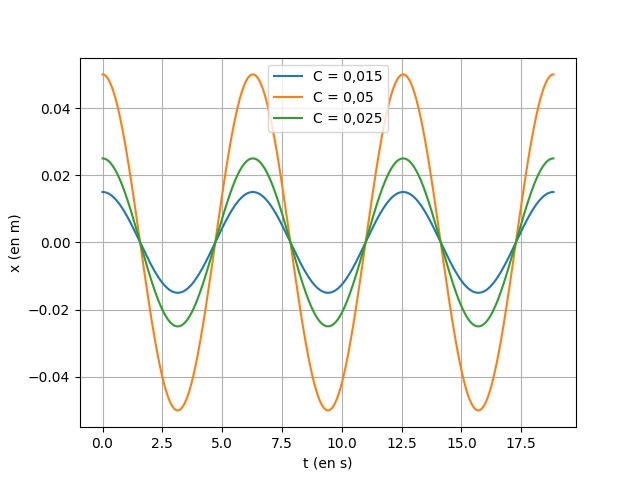
\includegraphics[width=.75\linewidth]{Figure_3.png}\end{center}
\begin{choices}
\correctchoice{6,25 secondes}
\wrongchoice{6,25 Hz}
\wrongchoice{12,5 secondes}
\wrongchoice{12,25 Hz}
\wrongchoice{0,015 , 0,05 , et 0,025 respectivement}
\end{choices}
\end{questionmult}
}
\element{grB}{
\begin{questionmult}{Q002}\scoring{haut=2}
Que peut-on dire pour le mouvement d'un système masse ressort horizontal présenté ci-dessous ?
\begin{center}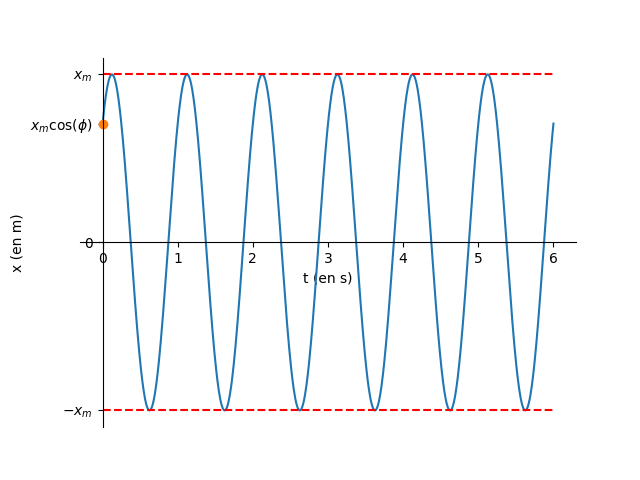
\includegraphics[width=.75\linewidth]{Figure_7.png}\end{center}
\begin{choices}
\correctchoice{La vitesse initiale est non nulle}
\correctchoice{L'origine de l'axe des X a été pris à la position d'équilibre}
\correctchoice{Il n'y a pas de frottements car l'amplitude ne diminue pas}
\correctchoice{La fréquence est de l'ordre de 1 Hz}
\correctchoice{Si on augmentait la masse, toutes choses égales par ailleurs, la pulsation propre du système diminuerait}
\end{choices}
\end{questionmult}
}
\element{grB}{
\begin{questionmult}{Q003}\scoring{haut=2}
Quelle est l'expression de l'énergie cinétique au cours du temps pour un système masse ressort horizontal ?
\begin{choices}
\correctchoice{$Ec(t)\ =\ \frac{1}{2} m {x_m}^2 {\omega_0}^2 \sin(\omega_0 t + \phi)$}
\wrongchoice{$Ec(t)\ =\ \frac{1}{2} m {x_m}^2 {\omega_0}^2 \cos(\omega_0 t + \phi)$}
\wrongchoice{$Ec(t)\ =\ \frac{1}{2} m {x_0}^2 {\omega_0}^2 \sin(\phi)$}
\wrongchoice{$Ec(t)\ =\ \frac{1}{2} m {x_m}^2 {\omega_0}^2 \sin(\phi)$}
\wrongchoice{$Ec(t)\ =\ \frac{1}{2} m {x_0}^2 {\omega_0}^2 \cos(\omega_0 t + \phi)$}
\end{choices}
\end{questionmult}
}
\element{grB}{
\begin{questionmult}{Q004}\scoring{haut=2}
Que peut-on dire de l'énergie mécanique d'un système masse ressort horizontal pour lequel on néglige les frottements
\begin{choices}
\correctchoice{L'énergie mécanique est conservée}
\correctchoice{L'énergie mécanique est répartie équitablement en moyenne entre énergie cinétique et énergie potentielle élastique}
\correctchoice{Elle est égale à $\frac{1}{2} k {x_0}^2\ +\ \frac{1}{2} m {v_0}^2$}
\correctchoice{Elle est égale à $\frac{1}{2} k {x(t)}^2\ +\ \frac{1}{2} m {v(t)}^2$}
\end{choices}
\end{questionmult}
}
\element{grB}{
\begin{questionmult}{Q005}\scoring{haut=2}
L'expression de $\omega_0$ pour un système masse ressort horizontal est
\begin{choices}
\wrongchoice{$\frac{k}{m}$}
\correctchoice{$\sqrt{\frac{k}{m}}$}
\correctchoice{$2 \pi f_0$}
\correctchoice{$\frac{2 \pi}{T_0}$}
\wrongchoice{$\frac{1}{2 \pi} \sqrt{\frac{k}{m}}$}
\wrongchoice{$\sqrt{\frac{m}{k}}$}
\wrongchoice{$2 \pi \sqrt{\frac{m}{k}}$}
\end{choices}
\end{questionmult}
}
\element{grB}{
\begin{questionmult}{Q006}\scoring{haut=2}
Quelle est la position d'équilibre pour un système masse ressort horizontal ?
\begin{choices}
\correctchoice{$l_{eq}\ =\ l_0$}
\wrongchoice{$l_{eq}\ <\ l_0$}
\wrongchoice{Cela dépend de la vitesse initiale}
\wrongchoice{Cela dépend de la position initiale}
\end{choices}
\end{questionmult}
}
\element{grB}{
\begin{questionmult}{Q007}\scoring{haut=2}
Quels sont les trois points à préciser avant de démarrer un exercice ?
\begin{choices}
\correctchoice{Le Système}
\correctchoice{Le référentiel}
\correctchoice{Le bilan des forces}
\wrongchoice{L'heure de début d'expérience}
\wrongchoice{La position d'équilibre du système}
\wrongchoice{La quantité de mouvement du système}
\end{choices}
\end{questionmult}
}
\element{grB}{
\begin{questionmult}{Q008}\scoring{haut=2}
Quelle est l'équation différentielle qui régit un oscillateur harmonique ?
\begin{choices}
\correctchoice{$\ddot{u}\ +\ {\omega_0}^2 u\ =\ 0$}
\wrongchoice{toute équation différentielle linéaire d'ordre 2}
\wrongchoice{$a x^2\ +\ b x\ +\ c\ =\ 0$}
\correctchoice{$\frac{d^2 x}{dt^2}(t)\ =\ -{\omega_0}^2 x(t)$}
\end{choices}
\end{questionmult}
}
\element{grB}{
\begin{questionmult}{Q009}\scoring{haut=2}
Quelle est l'expression de $x(t)$ pour un système masse ressort horizontal ?
\begin{choices}
\correctchoice{$x(t)\ =\ x_m \cos(\omega_0 t\ +\ \phi)$}
\wrongchoice{$x(t)\ =\ x_m \cos(\phi)$}
\correctchoice{$x(t)\ =\ A \cos(\sqrt{\frac{k}{m}} t)\ +\ B \sin(\sqrt{\frac{k}{m}} t)$}
\correctchoice{$x(t)\ =\ x_0 \cos(\omega_0 t)\ +\ \frac{v_0}{\omega_0} \sin(\omega_0 t)$}
\wrongchoice{$x(t)\ =\ \sqrt{{x_0}^2\ +\ \frac{{v_0}^2}{{\omega_0}^2}} \cos(\phi)$}
\correctchoice{$x(t)\ =\ \sqrt{{x_0}^2\ +\ \frac{{v_0}^2}{{\omega_0}^2}} \cos(\omega_0 t\ +\ \phi)$}
\end{choices}
\end{questionmult}
}
\def\insertPlainGroupgrB{\insertgroup{grB}}
\onecopy{5}{
\begin{center}\bf\large Essai de QCM\end{center}

{\setlength{\parindent}{0pt}\hspace*{\fill}\hbox{\vtop{\AMCcodeH{student.number}{2}}}\hspace*{\fill}\begin{minipage}[t]{5.8cm}$\longleftarrow{}$\hspace{0pt plus 1cm}Coder votre numero d'étudiant ici\vspace{3ex}

\hfill\namefield{\fbox{\begin{minipage}{.9\linewidth}\AMClocalized{namesurname}

\vspace*{.5em}\dotfill

\vspace*{.5em}\dotfill
\vspace*{1mm}
\end{minipage}
}}\hfill\vspace{5ex}\end{minipage}\hspace*{\fill}

}\vspace{4mm}
Veuillez cocher la ou les bonnes réponses. Les questions marquées d'un \multiSymbole{} comporte une ou plusieurs bonnes réponses. Les autres n'ont qu'une seule réponse possible.

\vspace{4mm}\noindent\hrule


\shufflegroup{grB}
\begin{multicols}{2}
\insertPlainGroupgrB
\end{multicols}


}
\end{document}
